\section{ Solving probleme by search}
\subsection{Structure d'un agent}
	Un agent est composé de 2 partie :
	\begin{itemize}
		\item \textbf{Architecture} : c'est les composants de l'ordinateur sur le quelle l'agent tourne
		\item \textbf{Programme} : Se sont les fonctions qui Map les perceptions en actions
	\end{itemize}
	
	Exemple d'un programme d'agent:
	
	\begin{itemize}
		\item Table de conduite de l'agent (\textbf{table driven})\\
		\item \textbf{Successor} : Tous les states atteignable depuis le state actuelle\\
		\item \textbf{Path} : Séquence de states connecté par une sequence d'action\\
		\item \textbf{Operators} : Manière de modifier un state avec une action\\
		\item \textbf{Goals Test} : Fonction qui teste si un state est le résultat final\\
		\item \textbf{Step Cost} : Cout numérique de passer du state $s$ avec l'action $a$ pour passer au state $s'$\\
		\item \textbf{Path Cost} : Fonction qui donne un cout a chaque path\\
		\item \textbf{Solution} : Séquence d'action de l'initial state jusqu'au goal state\\
		\item \textbf{Optimal Solution} : Solution avec le path avec le plus petit cout parmi toutes les solutions\\
		\item \textbf{Node} : Data structure qui constitue les graph et arbre de recherche\\
		\item \textbf{Frontier} : Ensemble de Node généré au quelle les ancêtre on été Goal-tested (visited)\\
		
		\item \textit{C'étais long mais bon fallait le faire}
		
	\end{itemize}
	\subsection{Problem solving Agent}
		\subsubsection{Definition Probleme}
			Un problème peut être définie avec :
			\begin{enumerate}
				\item States ou Initial State
				\item Une description des actions possible et valide par l'agent
				\item Une description de quoi chaque action fait (transition model)
				\item Un Goal test
				\item Un Path cost qui utilise un step cost
			\end{enumerate}
		\subsubsection{Solution}
			Une solution est une séquence d'action qui commence du state initial et qui termine à un des goal state. La solution est optimal si elle a la plus petite path cost parmis toutes les solutions
		\subsubsection{State space}
			Ensemble qui représente le problème avec les actions, les couts, ... (graph représentation). Possibilité d'un ensemble infini de states.
			\begin{figure}[htp]
				\centering
				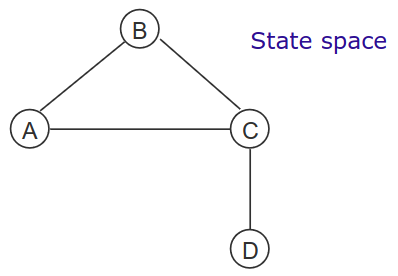
\includegraphics[width=.5\textwidth]{img/StateSpace.png}
			\end{figure}
		\subsubsection{Search Tree}
			Représentation du problème sous la forme d'arbre, avec les path entre les states et les goals. multiple path. Et un seul path d'un node a la racine.
			\begin{figure}[htp]
				\centering
				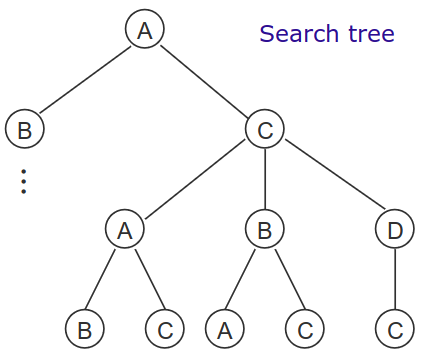
\includegraphics[width=.5\textwidth]{img/SearchTree.png}
			\end{figure}
			
		\subsubsection{State and Nodes}
			\begin{itemize}
				\item \textbf{State} représentation d'un configuration physique qui represente un state intermédiaire.
				\item \textbf{Node} data structure qui constitue le search tree
			\end{itemize}
			il peut y avoir plusieurs nodes avec le même state
		\subsubsection{Repeated States}
			On va éviter de visiter des Nodes qui on déjà été visité avant, pour cela, on va utiliser la représentation en arbre (search tree) et on ne pas va \textit{Expand} les nodes déjà visité.
	\subsection{Searching for Solutions}
		Trouver une solution est le fait de traverser un state space (graph ou tree) et du initial state au goal state avec un ensemble d'actions valide.


		\textbf{Expanding} : appliquer chaque action légal au state actuel.
		\begin{figure}[htp]
			\centering
			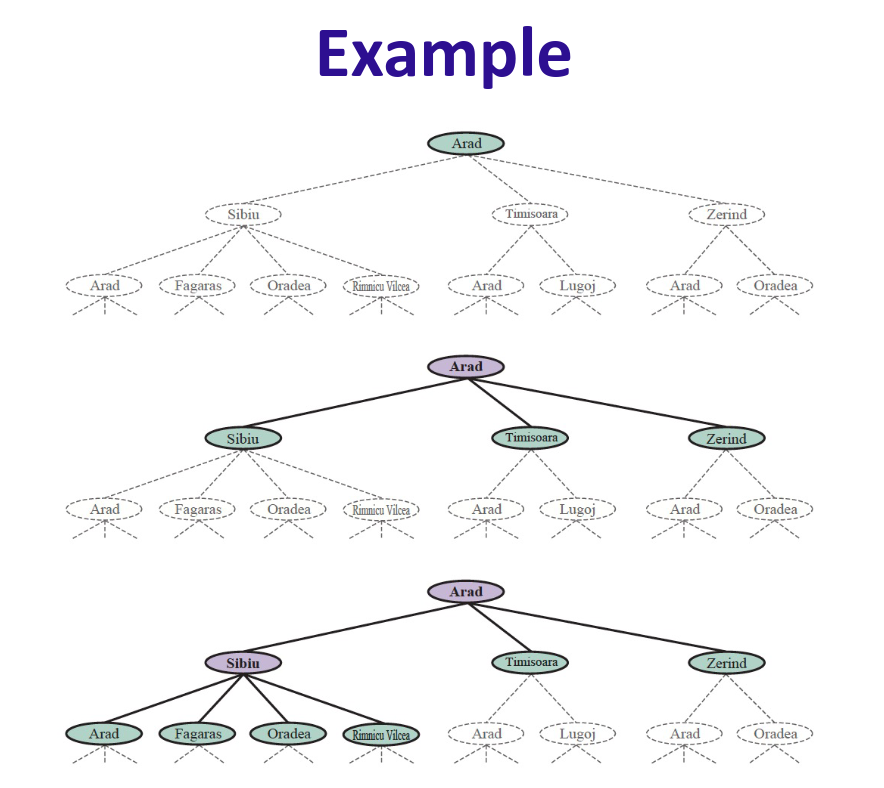
\includegraphics[width=0.6\textwidth]{img/ExempleExpanding.png}
		\end{figure}
		
		\textbf{Frontier} : Ensemble des node non-Expanded au quelle les ancêtres on déjà été visité. La frontière peut être représenté grâce a une Data structure Queue (lol zizi), On peut utiliser un Priority, LIFO, FIFO, \dots
		\begin{figure}[htp]
			\centering
			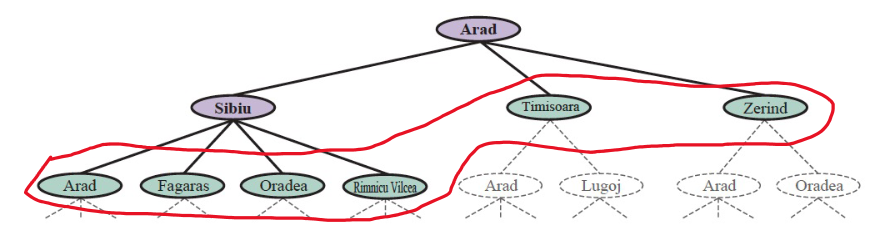
\includegraphics[width=0.6\textwidth]{img/FrontierExemple.png}
		\end{figure}
		
		\subsubsection{Stratégies}
			Il y a 2 types de recherches: 
			\begin{enumerate}
				\item \textbf{uninformed search} où la seul information de l'agent est \textit{"suis-je le but final ?"}.
				\item \textbf{informed search} où l'agent a les informations d'avant.
			\end{enumerate}
			
			On peut évaluer ces recherche avec 4 critères:
			\begin{itemize}
				\item \textbf{Completeness} : l'agent trouve un solution s'il en existe au moins une.
				\item \textbf{Time complexity} : Souvent en terme du nombre de nodes généré/Expanded
				\item \textbf{Space complexity} : Nombre de node en mémoire
				\item \textbf{Optimality} : Trouve solution avec le cout minimal 
			\end{itemize}
			
			On va utiliser 3 variables :
			\begin{itemize}
				\item \textbf{b} : Facteur de branchement maximal du Search tree
				\item \textbf{d} : Profondeur de la solution la moins couteuse
				\item \textbf{m} : Profondeur max de l'arbre (peut etre $\infty$)
			\end{itemize}
			
			\begin{figure}[H]
				\centering
				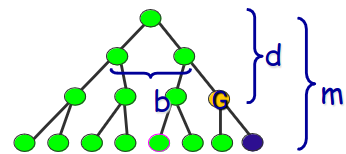
\includegraphics[width=.5\textwidth]{img/BDM.png}
			\end{figure}
	\subsection{Uninformed Search}
		\begin{figure}[htp]
			\centering
			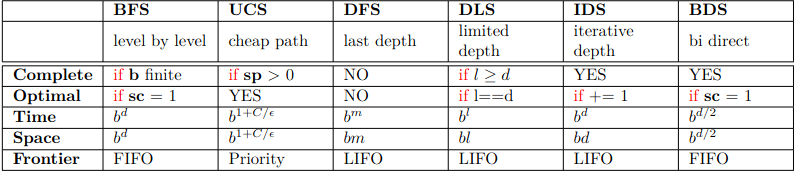
\includegraphics[width=\textwidth]{img/UninformedSearch.png}
		\end{figure}
		\subsubsection{Breadth-First Search(BFS)}
			Le but est de vérifier par niveau de l'arbre. Problème la mémoire est vite remplie. On commence du root node et ensuite on passe au sub-nodes qui sont dans une FIFO Queue qui représente la frontière.
			
			\begin{itemize}
				\item \textbf{Complétude} : Oui
				\item \textbf{Complexité temporelle} : $\mathcal{O}(b^d)$\footnote{$1+b+b^2 + \dots + b^d$}
				\item \textbf{Complexité spatiale} : $\mathcal{O}(b^d)$
				\item \textbf{Optimal} : Oui si cout = 1 (pas souvent le cas)
			\end{itemize}
			
			\begin{figure}[htp]
				\centering
				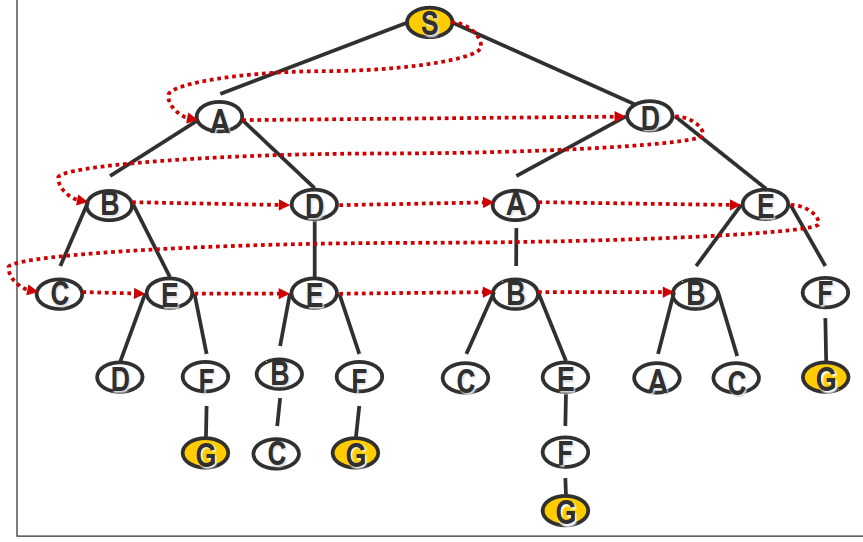
\includegraphics[width=0.6\textwidth]{img/BFS.png}
				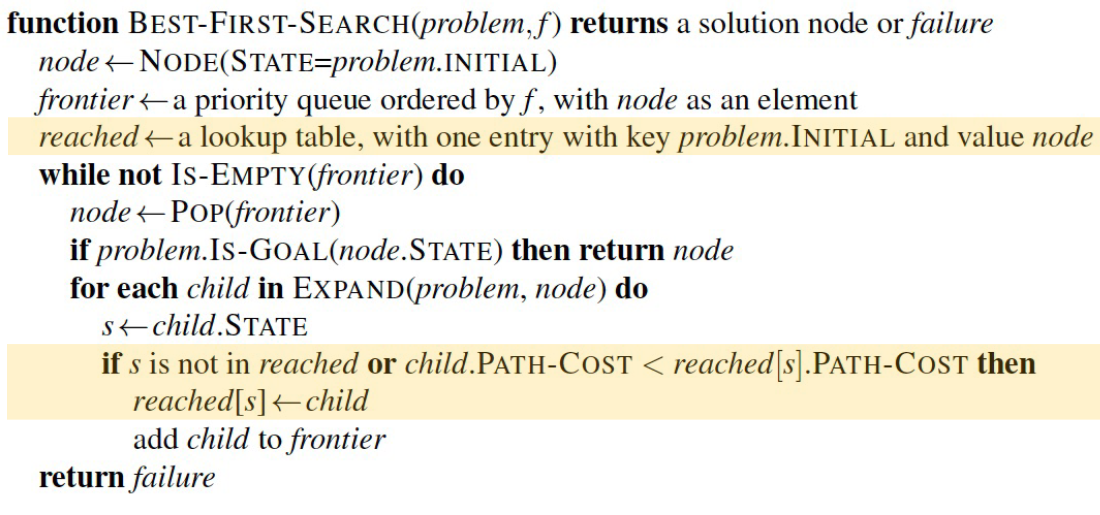
\includegraphics[width=\textwidth]{img/CodeBFS.png}
			\end{figure}					
		\newpage
		\subsubsection{Uniform-Cost search (UCS)}
			Comme le BFS sauf que le Node avec le cout le plus petit est exploré en premier. Il y a un cout pour passer d'un node a l'autre. La frontière est implémenté avec un Priorety Queue. Fort semblable a Dijkstra.
			
			\begin{figure}[htp]
				\centering
				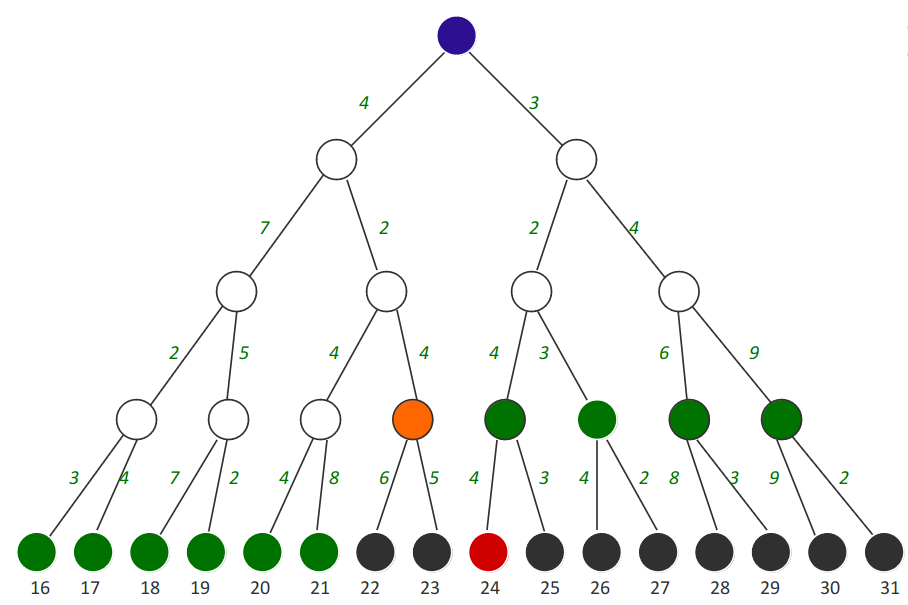
\includegraphics[width=0.6\textwidth]{img/UCS.png}
			\end{figure}
			
			\begin{itemize}
				\item \textbf{Completude} : Si cout strictement positif ($\geq \epsilon \geq 0$)
				\item \textbf{Complexité temporelle} : Dure a dire
				\item \textbf{Compelxité spatiale} : $\mathcal{O}(b^{C^{*/\epsilon}}$
				\item \textbf{Optimal} : Oui
			\end{itemize}
			
			
			
		\subsubsection{Depth-first Search (DFS)}
		Concrètement, on visite toutes une branche de l'arbre jusqu'à arriver à la \textit{Leaf}, si on ne trouve pas le goal on passe a la prochaine, etc.
		La Frontière est implémenté avec un Queue LIFO.
		
		\begin{itemize}
			\item \textbf{Complétude} : Non car peut avoir profondeur (m) $\infty$
			\item \textbf{Complexité temporelle} : $\mathcal{O}(b^m)$ mauvais si ($m > d$)
			\item \textbf{Complexité spatiale} : $\mathcal{O}(mb)$
			\item \textit{Optimal} : Non
		\end{itemize}
		
		\begin{figure}[htp]
			\centering
			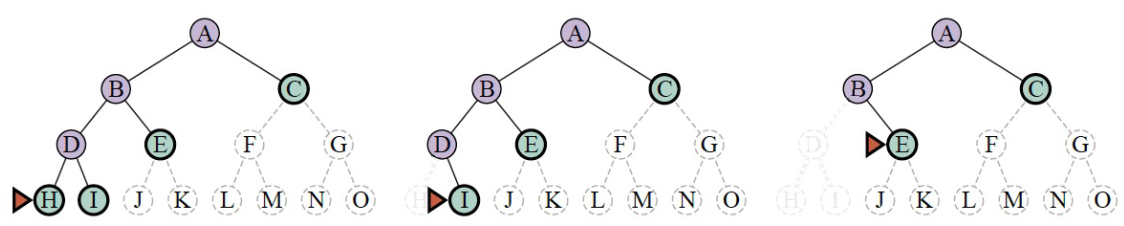
\includegraphics[width=\textwidth]{img/ExempleDFS.png}
		\end{figure}
		
		\subsubsection{Depth-Limited Search}
			Pareil de DFS sauf que la on met une limite de profondeur(depth) $l$.
		
		\subsubsection{Iterative Deepening}		
		  Pareil que DLS mais si $l < d$ alors on ne trouveras jamais de solutions, donc on va incrémenter petit a petit $l$
			\begin{figure}[htp]
				\centering
				$l = 1$
				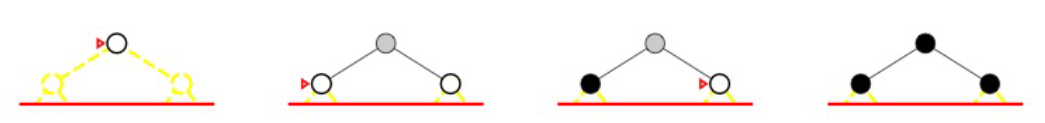
\includegraphics[width=\textwidth]{img/DLS1.png}
				$l = 2$
				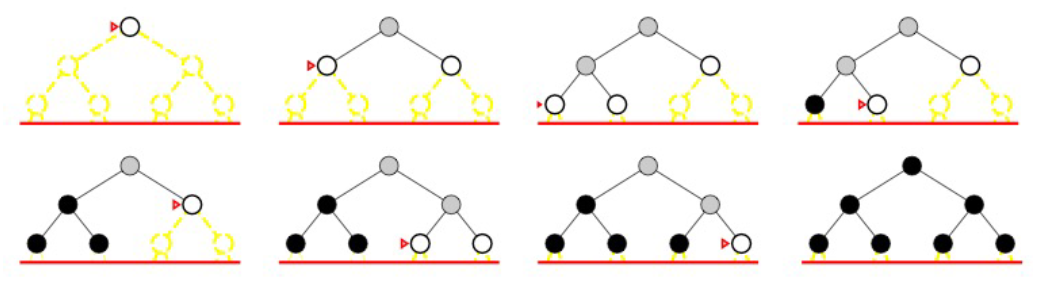
\includegraphics[width=\textwidth]{img/DLS2.png}
				$l = 3$
				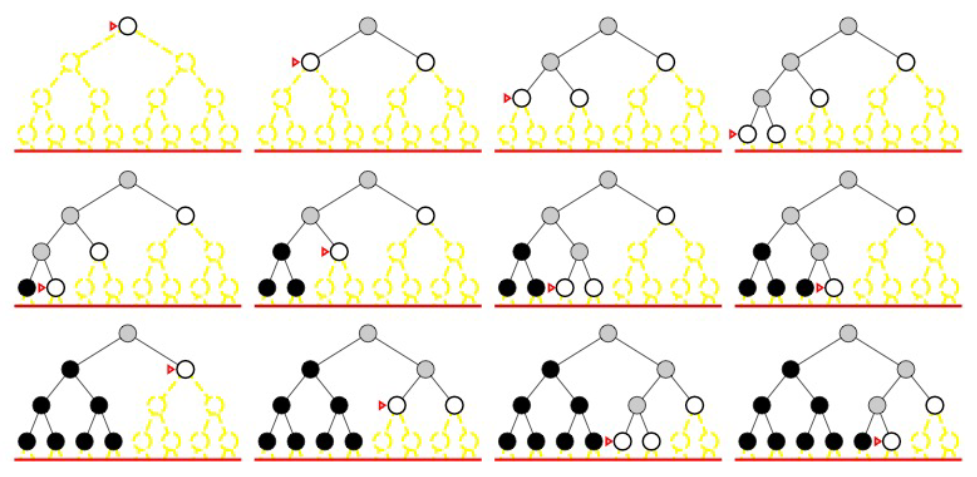
\includegraphics[width=\textwidth]{img/DLS3.png}

			\end{figure}
			
		Plusieurs nodes sont visité plusieurs fois, mais ce n'est pas très grave car il n'y en a pas beaucoup.
		
		\begin{itemize}
			\item \textbf{Complétude} : Oui
			\item \textbf{Complexité temporelle} : $\mathcal{O}(b^d)$
			\item \textbf{Complexité spatiale} : $\mathcal{O}(b^d)$
			\item \textbf{Complétude} : Oui si cout = 1
		\end{itemize}
		
		
		\subsubsection{Biderectional Search}
			On commence du root jusqu'au Goal et aussi du Goal jusqu'au root et on stoppe quand les 2 s'intersecte. Il y quelque difficulté.
			\begin{itemize}
				\item Prédécesseurs du goal doivent être généré (pas toujours possible)
				\item Search doit être coordonnée entre les 2 recherches
				\item Problème si plusieurs Goal
				\item Tous les nodes doivent rester en mémoire
			\end{itemize}
			
			\begin{itemize}
				\item \textbf{Complétude} : Oui
				\item \textbf{Complexité temporelle} : $\mathcal{O}(b^{d/2})$
				\item \textbf{Complexité spatiale} : $\mathcal{O}(b^{d/2})$
				\item \textbf{Optimal} : Oui si cout = 1
			\end{itemize}
			
	\subsection{Informed Search}
		En utilisant des connaissances spécifiques au problème, trouver et/ou déduire des informations sur les States futurs et les paths futures.
		
		BFS est un algo de recherche ou les nodes sont sélectionner pour êtres \textit{Expand} basé sur \textbf{une fonction d'évaluation} $f(n)$, cela donne un cout et on choisi le node avec le plus petit cout avec une Priority Queue.
		
		Attention on calcule une évaluation et non pas la distance exacte
		
		\subsubsection{Heuristic Fonction}
		
		Noté $h(n)$ est une fonction qui estime le cout d'un node vers le goal. c'est une approximation car on ne connait pas le cout exacte.
		\begin{figure}[htp]
			\centering
			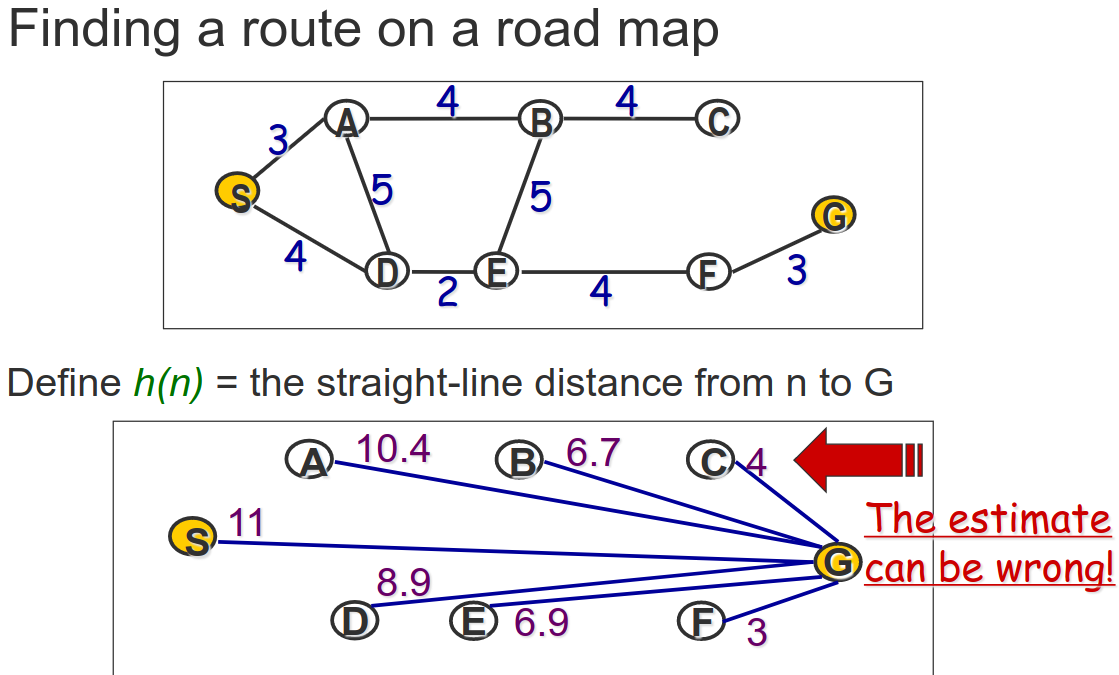
\includegraphics[width=0.8\textwidth]{img/ExempleHeuristic.png}

		\end{figure}
		
		Il y a 3 types de fonction Heuristique :
		\begin{itemize}
			\item \textbf{Optimistic} : Admissible car elle pense que le cout pour résoudre le problème est inférieur au cout réel
			\item \textbf{Admissible} : Ne surestime jamais le cout pour atteindre le goal. Le cout qu'il estime est plus grand que le plus petit cout possible par rapport au node actuel. $h(n) = 0$ si c'est un Goal state.
			\item \textbf{Consistent} : L'estimation de un node $n$ au goal est plus petit que le cout réel de $n$ a un nouveau node $n'$ avec l'action $a$ plus l'estimation de $n'$ au goal 
			\begin{equation}
				h(n) \leq c(n,a,n') + h(n')
			\end{equation}
		\end{itemize}
		
		un consistent heuristi est admissible
		
		\subsubsection{Triangle inequality}
			\begin{figure}[htp]
				\centering
				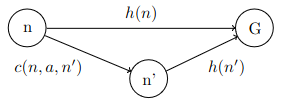
\includegraphics[scale=1]{img/Triangle.png}
			\end{figure}
			Chaque coté du triangle ne peut pas être plus long que la somme des autres cotés.
			\begin{itemize}
				\item \textbf{h(n)} : Estime le cout entre $n$ et $G$
				\item \textbf{C(n,a,n')} : cout pour aller en $n'$ depuis $n$ avec l'action $a$
				\item \textbf{h(n')} : cout estimé entre $n'$ et $G$
			\end{itemize}
			
		\subsubsection{Monotonicity} 
			Si $h(n)$ est consistant alors f(n) le long d'un path quelconque n'est pas décroissant. Supposons que $n'$ est un successeur de $n$ alors :
			
			\begin{figure}[htp]
				\centering
				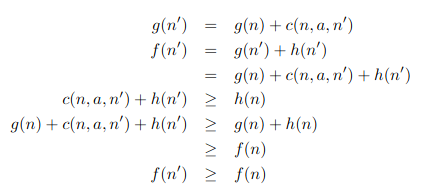
\includegraphics[scale=1]{img/Monotonicité.png}
			\end{figure}
		\subsubsection{Greedy Best-First Search(GBFS)}
			Tente d'étendre le node qui est le plus proche du Goal. Donc ici, $f(n) = h(n)$
						
			\begin{itemize}
				\item \textbf{Complétude} : Non, profondeur peut etre infinie
				\item \textbf{Complexité temporelle} : $\mathcal{O}(b^m)$
				\item \textbf{Complexité spatiale} : $\mathcal{O}(b^m)$
				\item \textbf{Optimal} : Non
			\end{itemize}
			
			\begin{figure}[htp]
				\centering
				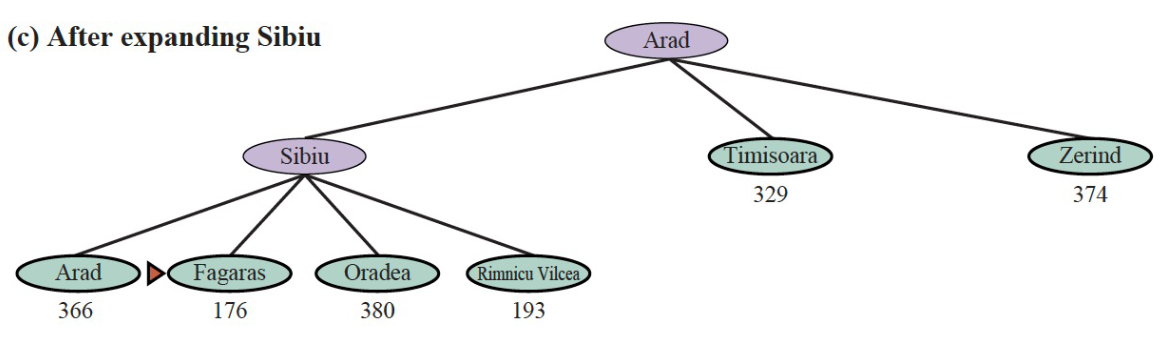
\includegraphics[width=\textwidth]{img/GBFS.png}
			\end{figure}
			
		\subsubsection{A*}
		Fusion de GBFS et Uniform cost. Minimise le cout total estimé de la solution
		
		\begin{figure}[H]
			\centering
			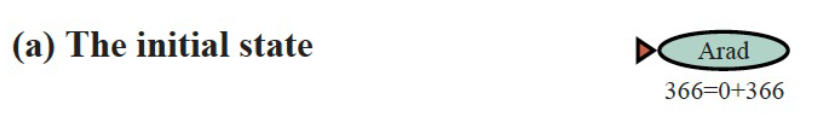
\includegraphics[width=\textwidth]{img/A.png}
		\end{figure}
		\begin{figure}[H]
			\centering
			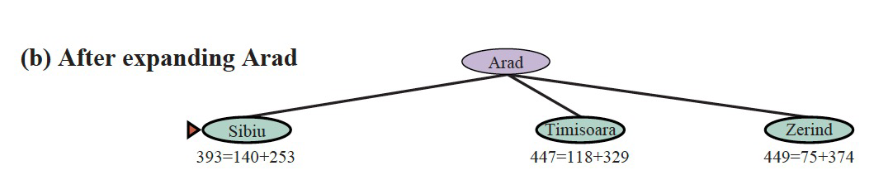
\includegraphics[width=\textwidth]{img/A1.png}
		\end{figure}\begin{figure}[H]
			\centering
			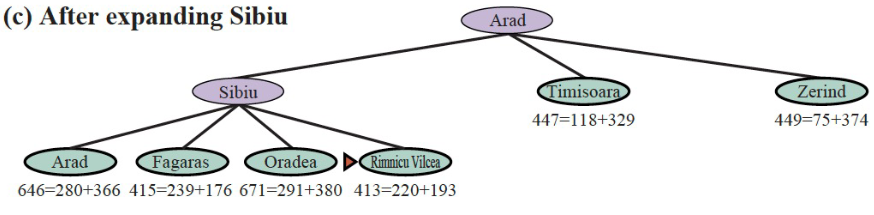
\includegraphics[width=\textwidth]{img/A2.png}
		\end{figure}\begin{figure}[H]
			\centering
			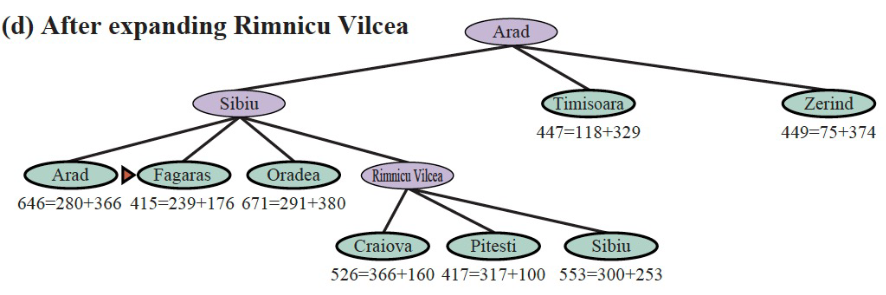
\includegraphics[width=\textwidth]{img/A3.png}
		\end{figure}\begin{figure}[H]
			\centering
			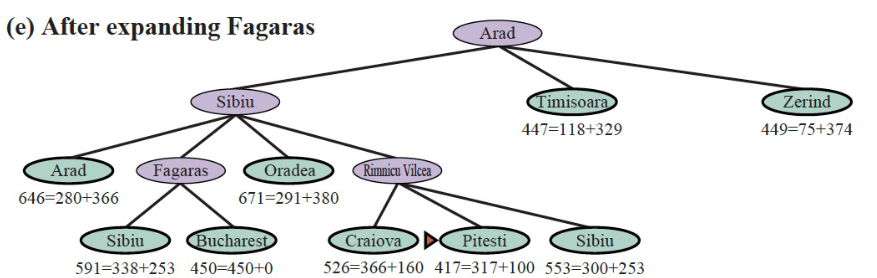
\includegraphics[width=\textwidth]{img/A4.png}
		\end{figure}\begin{figure}[H]
			\centering
			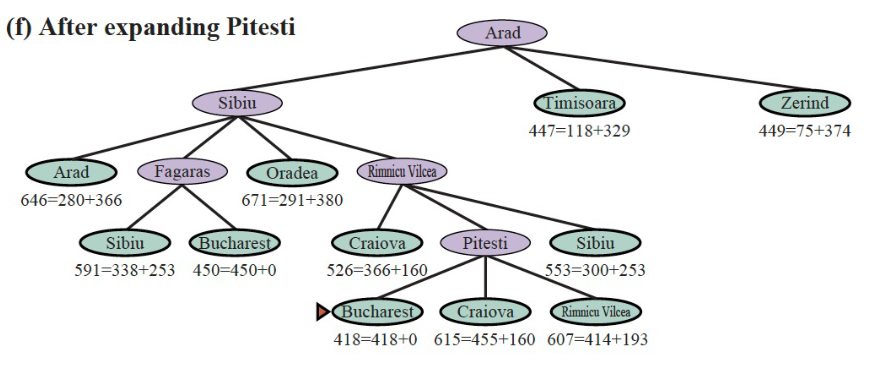
\includegraphics[width=\textwidth]{img/A5.png}
		\end{figure}
		
		\begin{equation}
			f(n) = g(n) + h(n)
		\end{equation}
		
		Avec $g(n)$ le cout du chemin du state initial au node $n$ et $h(n)$ l'heuristique qui approxime le cout du chemin du node $n$ vers le goal.
		
		$g(n)$ est donc un valeur calculé alors que $h(n)$ n'est qu'une approximation.
		
		$h(n)$ ne doit pas surestimer le cout vers le goal
		
		On peut prouver que si A* est optimal si $h(n)$ est admissible.
		
		\textbf{Preuve :}
		\begin{itemize}
			\item Une solutions est chemin initial $\rightarrow$ goal
			\item On pose $C^*$ le chemin a cout minimal
			\item On doit montrer que $A*$ ne retroune pas une chemin suboptimal (une solutions mais pas avec le chemin le plus court)
			\item \textbf{Partie 1}
			\begin{itemize}
				\item $G$ est un goal suboptimal de la frontière
				\item path cost $g(G) = C$ avec $C > C^*$
				\item $h(G) = 0$
				\item $f(G) = g(G) = C > C^* \Leftrightarrow f(G) > C^*$
			\end{itemize}
			\item \textbf{Partie 2}
			\begin{itemize}
				\item $n$ est un node sur le chemin optimal
				\item $f(n) = g(n) + h(n)$
				\item $f(n) \leq C^*$
			\end{itemize}
			\item \textbf{Partie 3}
			\begin{itemize}
				\item $f(n) \leq C^* < f(G)$
				\item Node $G$ ne sera jamais choisis $\Rightarrow$ \textbf{CQFD}
			\end{itemize}
		\end{itemize}
		
			
		Monotonicité de $f(n)$
		\begin{itemize}
			\item Avec $h(n)$ consistent, alors $f(n)$ le long de n'importe quel  chemin est non décroissant (\textbf{Monotonicité})
			\begin{itemize}
				\item On suppose $n'$ successeur de $n$
				\begin{itemize}
					\item $g(n') = g(n) + c(n,a,n')$
					\item $f(n') = g(n') + h(n') = g(n) + c(n,a,n') + h(n')$
					\item Par la consistance, $h(n) \leq c(n,a,n') + h(n')$
					\item $f(n') \geq g(n) + h(n) = f(n)$
					\item $f(n') \geq f(n)$ 
				\end{itemize}
			\end{itemize}
		\end{itemize}
		
		\Large{\textbf{Search Contours}} \normalsize
		
	
			un \textbf{Contour} c'est un groupe de node avec $f(n)$ < une certaine valeur
			
			Le problème de mémoire de A* est a cause que il s'ented de la meme maniere qu'un BFS qui s'etend par courche et A* par f-contours.
			
			\begin{figure}[H]
				\centering
				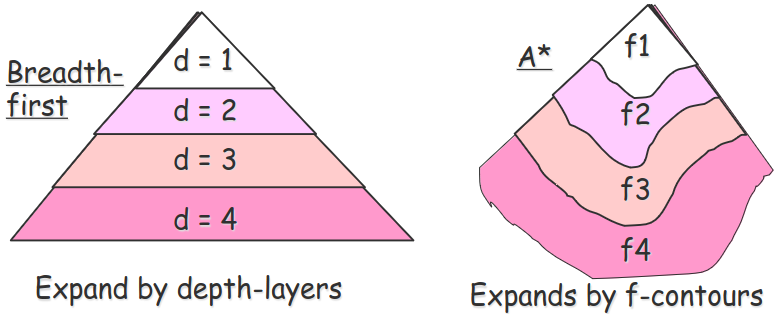
\includegraphics[width=\textwidth]{img/MPA}
			\end{figure}			 
		
			A* étant donc tous les nodes $f(n) < C^*$ et il étand au moins un node du contour $C^*$ avant de trouver le goal.
		
			A* est "optimalement efficace" en utilsnat le graph search car il étend le moins de node
			
			\textbf{Proprités}
			\begin{itemize}
				\item \textbf{Complétude} : Oui
				\item \textbf{Complexité temporelle} : $\mathcal{O}(b^d)$
				\item \textbf{Complexité spatiale} : $\mathcal{O}(b^d)$
				\item \textbf{Optimal} : Oui
			\end{itemize}
			
			Pour réduire le nombre de nodes visité, on peut choisir de pas choisir le node le plus optimal et prendre un suboptimal en utilisant un heuristique pas admissible.
			
			On peut aussi faire en sorte d'utiliser toutes la mémoire disponnible et si on est plein, on décide de retirer les nodes "inutile".
			
		\subsubsection{Weighted A*}
			
			\begin{equation}
				f(n) = g(n) + w.h(n) (\text{avec} w>1)
			\end{equation}
			
			La solution est garantie d'etre dans un interval constant de facteur $w$ de la solution optimal
			
			\begin{center}
			\begin{tabular}{|c|c|c|}
				\hline
				$A*$ & $g(n) + h(n)$ & $w=1$\\ \hline
				Unifirm-cost & $g(n)$ & $w=0$ \\ \hline
				Greedy best-first & $h(n)$ & $w=\infty$ \\ \hline
				Weighted $A*$ & $g(n)+w.h(n)$ & $1<w<\infty$\\ \hline
			\end{tabular}
			\end{center}
			
		\subsubsection{Iterative deepening A*}
			A* avec une limite de depth $l$ qui est incrémenté itérativement.
			
			IDA* expend seulement les nodes avec f-cost() $\leq$ que les nodes non expand a la dernière itérations.
		
			Ce n'est pas efficace quand le nombre des f-cost() sont élevés.
			
			Propriétés :
			\begin{itemize}
				\item \textbf{Complet} : Oui
				\item \textbf{Time complexity} : exponentiel
				\item \textbf{Space complexity} : Linéaire
				\item \textbf{Optimal et $h()$ consistent}
				\item \textbf{Efficace si absence de monotonicité}
			\end{itemize}
			
		\subsubsection{Recursive Best-First Search}		
			DFS combiné avec une meilleur alternative :
			\begin{itemize}
				\item Garde en mémoire les options en marge
				\item Dés que current depth first exploration devient trop couteux, change en
			\end{itemize}
			
		\subsubsection{Simple Memory-Bounded A* (SMA*)}
		
			A* classique et on utilise toutes la mémoire disponible, déq que il y a plus de place, on retire celui avec la pire f-value pour mettre le nouveau
			
			Regénère un arbre de décision seulement quand nécessaire.
			
			\begin{itemize}
				\item \textbf{Complete}: oui si asser de mémoire pour le plus cour chemin
				\item \textbf{Optimal} : Oui si asser de place en mémoire pour stocker le path de la meilleur solutions
				\item \textbf{Complexité temporelle} : Meme que A*
				\item \textbf{Space complexity} : utilise ce qui est disponible

			\end{itemize}
			
			Souvent meilleur que A* et IDA* car bon compromis entre temps et espace
		
	
	\subsection{Heuristic en pratique}
		\subsubsection{Comparer 2 heuristique}	
			On compare le nombre total de node généré N
			
			On compare les arbres de recherches (effective branching factor $b*$)
			\begin{itemize}
				\item On réarrange les arbres en les rendent complet pour les rendre comparables
				\item $b*$ d'un arbre de depth $d$ contient N+1 nodes
			\end{itemize}
			
			Le meilleur heuristique est toujours le mieux informé
			
			$h_2$ sera toujour meilleur que $h_1$ temps que  :
			\begin{itemize}
				\item $\forall \text{node} n : h_2(n) \geq h_1(n)$
				\item $h_2$ domine $h_1$
			\end{itemize}
			
		\subsubsection{Desing d'heuristique admissible}
			Un technique est de simplifier le problème en retirant des restrictions sur les actions.
			
			Le cout de la solutions de ce problème simplifié est toujours une heuristique admissible du probleme original.